%%%%%%%%%%%%%%%%%%%%%%%%%%%%%%%%%%%%%%%%%%%%%%%%%%%%%%%%%%%%%%%%%%%%%%
%     File: ExtendedAbstract_backg.tex                               %
%     Tex Master: ExtendedAbstract.tex                               %
%%%%%%%%%%%%%%%%%%%%%%%%%%%%%%%%%%%%%%%%%%%%%%%%%%%%%%%%%%%%%%%%%%%%%%

\section{Related Work}
\label{sec:related}

Our approach builds upon RSRefSeg, a state-of-the-art architecture for referring segmentation that combines vision-language understanding with precise mask generation capabilities. As illustrated in Figure \ref{fig:rsrefseg_architecture}, RSRefSeg employs a dual-encoder approach utilizing SigLIP for text and image feature extraction, followed by SAM for high-quality segmentation mask generation. This architecture provides a robust foundation for our aerial imagery segmentation tasks by leveraging the strong pre-trained capabilities of both foundation models while enabling efficient adaptation through LoRA fine-tuning.

\begin{figure*}[t]
\centering
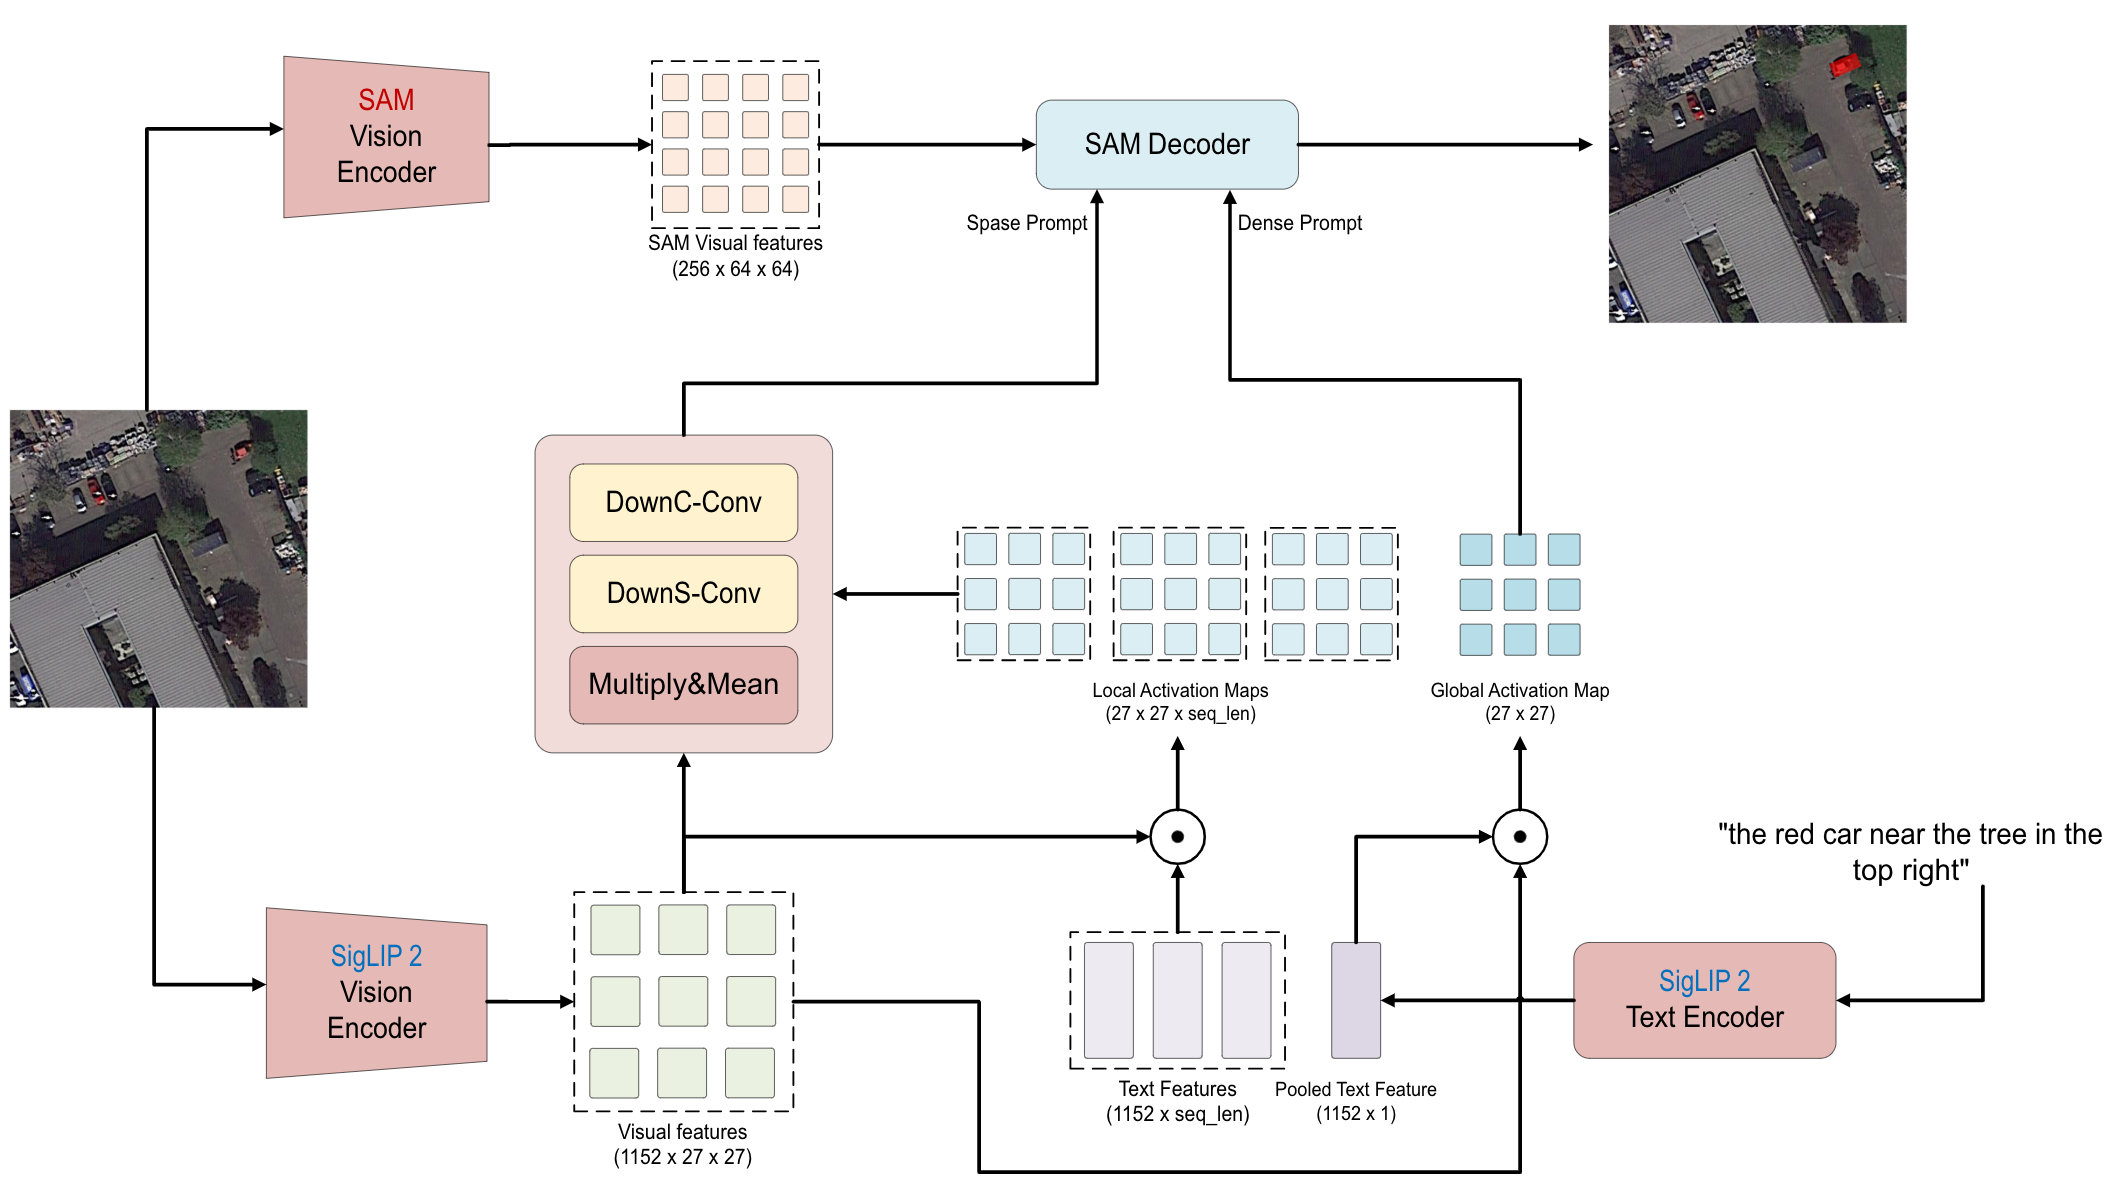
\includegraphics[width=0.85\textwidth]{./images/rsrefseg.png}
\caption{RSRefSeg architecture combining SigLIP text-image encoding with SAM mask generation for referring segmentation tasks.}
\label{fig:rsrefseg_architecture}
\end{figure*}

